\chapter{Tutorials}

It is assumed that the user has at least a working knowledge of the Python programming language including such concepts as `if' statements, `while' and `for' loops, `tuples', `lists' and `function/method calls'.  If this is not the case, we recommend the user take the Google Python Class (\url{https://developers.google.com/edu/python/}) or work through the official Python tutorials (\url{http://docs.python.org/2/tutorial/}), both of which are available free of charge.

%%%%%%%%%%%%
% Section: Biolecular %
%%%%%%%%%%%%
\section{A Simple Example: Bimolecular Reaction}

In the first tutorial, we will motivate stochastic modeling with a simple example of a bimolecular reaction among three low copy number molecular species.  First, we will use a traditional continuous ODE approach to solving the equations using the SciPy \texttt{odeint} function and then use pyLM and Lattice Microbes to simulate the same system.\\

We will simulate the association/dissociation reaction of hypothetical molecules:\\

\begin{centering}
\ce{A + B <=>[\ce{k_f}][\ce{k_r}]C}\\
\end{centering}

Writing out the differential equations will facilitate the ODE definition in SciPy:
\begin{align*}
\frac{d[A]}{dt}&=-k_f[A][B]+k_r[C]\\
\frac{d[B]}{dt}&=-k_f[A][B]+k_r[C]\\
\frac{d[C]}{dt}&=k_f[A][B]-k_r[C]
\end{align*}

Let us start out with a low number of each particles: 1000 of A and B and 0 of C.  Let us imagine simulating that problem in a microbe sized volume of 1 $fL$. Also, let us start off with rates of $k_f=1.07\times 10^5M^{-1}s^{-1}$ and $k_r=0.351/s$.  The Python script in Listing \ref{lst:bimolODE} will solve this using a deterministic solver.

\lstinputlisting[style=customPy, caption={\texttt{tut1.1-ODEBimol.py} --- Code used to solve the bimolecular reaction with a continuous ODE solver.}, backgroundcolor=\color{mygray}, label=lst:bimolODE]{CodeFiles/tut1.1-ODEBimol.py}

Running this code will create the plot shown in Figure \ref{fig:tut11}a.  Walking through the script, we start out defining some constants, followed by a definition of a function that returns the rates in the previous equations followed by a solve for 1 million different time points.  Finally the results are plotted.  Of particular note is the division of the forward rate constant by Avogadro's number and the volume of the cell which takes us to units of molecules per second.  This is the standard for stochastic simulations and will be described shortly.\\

What you should note about the results are that the count of each species varies smoothly across the time course.  However, it is reasonable to define molecules at their endpoints, either reactants or products, which necessarily means that the count of each molecule must be a whole number.  Furthermore, this implies that the count of the molecules changes in integer units.  Stochastic modeling was designed to address this point.  \\

\begin{figure}[h!]
  \centering
        \begin{subfigure}[b]{0.49\textwidth}
                \includegraphics[width=\textwidth]{Figures/BimolecularODE.png}
        \end{subfigure}
        \begin{subfigure}[b]{0.49\textwidth}
                \includegraphics[width=\textwidth]{Figures/BimolecularStoch.png}
        \end{subfigure}
        \caption{(a) A deterministic solution to the bimolecular reaction. (b) A stochastic solution to the bimolecular simulation.} \label{fig:tut11}
\end{figure}

Next, let us try doing the same simulation in Lattice Microbes.  The Python script in Listing \ref{lst:bimolLM} will accomplish this. To run the simulation, you should execute the command: 

\begin{verbatim}
python tut1.2-StochBimol.py
\end{verbatim}

The simulation will take from a few seconds to perhaps a minute to complete.\\

The first thing to note are the new import statements.  \texttt{pyLM} contains the main modules for setting up reactions.  \texttt{pyLM.units} contains helper functions for scaling numbers in a legible way.  \texttt{pySTDLM} is a library of standard functionality such as standard reaction systems, cell systems.  In addition it contains a number of pre- and post-processing functionality.  The net few lines are merely definitions of some constants.  The line \texttt{sim=CME.CMESimulation()} creates an empty simulation object. The next lines define the chemical species; in pyLM species are named by python strings and must be registered with the simulation using the \texttt{defineSpecies} command.  \\

The next two lines set up the reactions.  In Lattice Microbes all reactions are irreversible, necessitating the specification of both the forward and back reactions separately.  The first and second argument can be either a tuple of reactants or a string when only one reactant is specified.  Lattice Microbes currently supports 0th, 1st and 2nd order reactions, and reaction rates must be specified in the ``stochastic" format (see Table \ref{tbl:rxnTypes}). In the special case of a 0th order reaction, the empty string \texttt{''} should be passed as the reactant.  In addition, annihilation reactions can be specified by passing the empty string \texttt{''} as the product parameter.  \\

\begin{table}[htdp]
\begin{center}
\begin{tabular}{|c|c|c|c|c|}
\hline
\textbf{Order} & \textbf{Form} & \textbf{Parameters} & \textbf{Macroscopic Units} & \textbf{Stochastic Rate Constant ($s^{-1}$)}\\
\hline\hline
0th  & $\emptyset\rightarrow$A  & $k$ & $Ms^{-1}$ & $k\cdot V \cdot N_A$\\
\hline
1st & A$\rightarrow$B & $k$ & $s^{-1}$ & $k$ \\
\hline
2nd & A+B$\rightarrow$C & $k$ & $M^{-1}s^{-1}$ & $\frac{k}{V\cdot N_A}$ \\
\hline
2nd (Self) & 2A$\rightarrow$B & $k$ & $M^{-1}s^{-1}$ & $\frac{k}{V\cdot N_A}$ \\
\hline
\end{tabular}
\end{center}
\caption{Reactions available to both CME and RDME.  Here, the stochastic rate constant should be computed from the macroscopic rate constant (perhaps from experiment) using the volume of the experiment, $V$, and Avogadro's number, $N_A$.} \label{tbl:rxnTypes}
\end{table}%

The following lines merely define the initial species counts.  Next the simulation parameters are specified, time steps will be written out every 30 microseconds and the total simulation will run for 30 seconds.  The next line is of particular importance; the simulation {\emph must} be saved to a file before running the simulation.  Finally, we call the \texttt{run(...)} command on the simulation object giving it the name of the simulation file, the simulation method and the number of independent trajectories (replicates) to run of that simulation.  Finally, we use one of the post processing commands to look plot the time course of the $A$ and $C$ species for replicate number 1 (replicates are indexed starting at 1) into the file `BimolecularStoch.png'.  


\lstinputlisting[style=customPy, caption={\texttt{tut1.2-StochBimol.py} --- Code used to solve the bimolecular reaction with the discrete/stochastic Lattice Microbes CME implementation.}, backgroundcolor=\color{mygray}, label=lst:bimolLM]{CodeFiles/tut1.2-StochBimol.py}

One example of the output can be seen in Figure \ref{fig:tut11}. You might note that the behavior is qualitatively the same, however there appears to be considerable fluctuation, even after the system has come to equilibrium.  This is due to the stochastic nature of the process, where the reaction can transiently fluctuate away from the equilibrium value.  In addition, you may be able to tell that the changes in particle number from one time to another are in integer increments, though this will become considerably more obvious at lower number of particles. \\

To convince yourself that the system obeys the the macroscopic limit---or in other words the average over many realizations of the system trajectory will give back the continuous behavior---try modifying the last few lines of the script with the following and rerun: 

\begin{lstlisting}[style=customPy, backgroundcolor=\color{mygray}, label=lst:bimolLM]
sim.save('T1.3-bimol.lm')

# Run 100 replicates using the Gillespie solver
sim.run(filename='T1.3-bimol.lm', method="lm::cme::GillespieDSolver", replicates=100)

# Plot the solution
plotAvgVarFromFile(filename='T1.3-bimol.lm', species=['A','C'], outfile='BimolecularAvgVar.png')
\end{lstlisting}

The last command takes all of the replicates found in the simulation output, performs a time average over their species counts and computes the variance. You should see something similar to the plot in Figure \ref{fig:bimolRep}, Where the average appears to be the continuous limit but the variance is quite large. \\

\begin{figure}[h!]
  \centering
        \includegraphics[width=0.7\textwidth]{Figures/BimolecularAvgVar.png}
        \caption{Average over many independent trajectories sampling the stochastic equation.} \label{fig:bimolRep}
\end{figure}

So now that you have a working understanding of using the CME solver in pyLM try to answer the following:
\begin{enumerate}
\item How does initial particle count affect stochasticity?
\item How do the rates of reaction affect stochasticity?
\item What role does volume play in the reaction system?
\item What is the threshold where the continuous assumption of the ODE breaks down?
\item What happens to the fluctuations if you have competition for one of the reactants?  For example if you had another reaction like: \ce{A <=> D}
\end{enumerate}


%%%%%%%%%%%%%%%%
% Section: Lac 2 state switch %
%%%%%%%%%%%%%%%%
\section{Seeing is Believing: {\it lac} Genetic Switch}

The {\it lac} genetic switch in {\it E. coli} shows considerable stochasticity during the switch from utilizing glucose to lactose \cite{Roberts2011nci} (shown in Figure \ref{fig:lacSwitch}).  In monoclonal colonies growing in exponential phase that use up available glucose, the time for each cell to turn ``on" can vary by many minutes or even an hour depending on the availability of lactose and the number of repressor proteins that are present in the cell. To exacerbate this, the DNA for the gene is available in only one copy in the cell which can be ``on" or ``off" depending on if a repressor is bound, and affects downstream availability and number of mRNA and the protein.  The lifecycle of the system, upon addition of lactose (and depletion of the more favored glucose) is depicted in Figure \ref{fig:lacLife}.

\begin{figure}[h!]
  \centering
        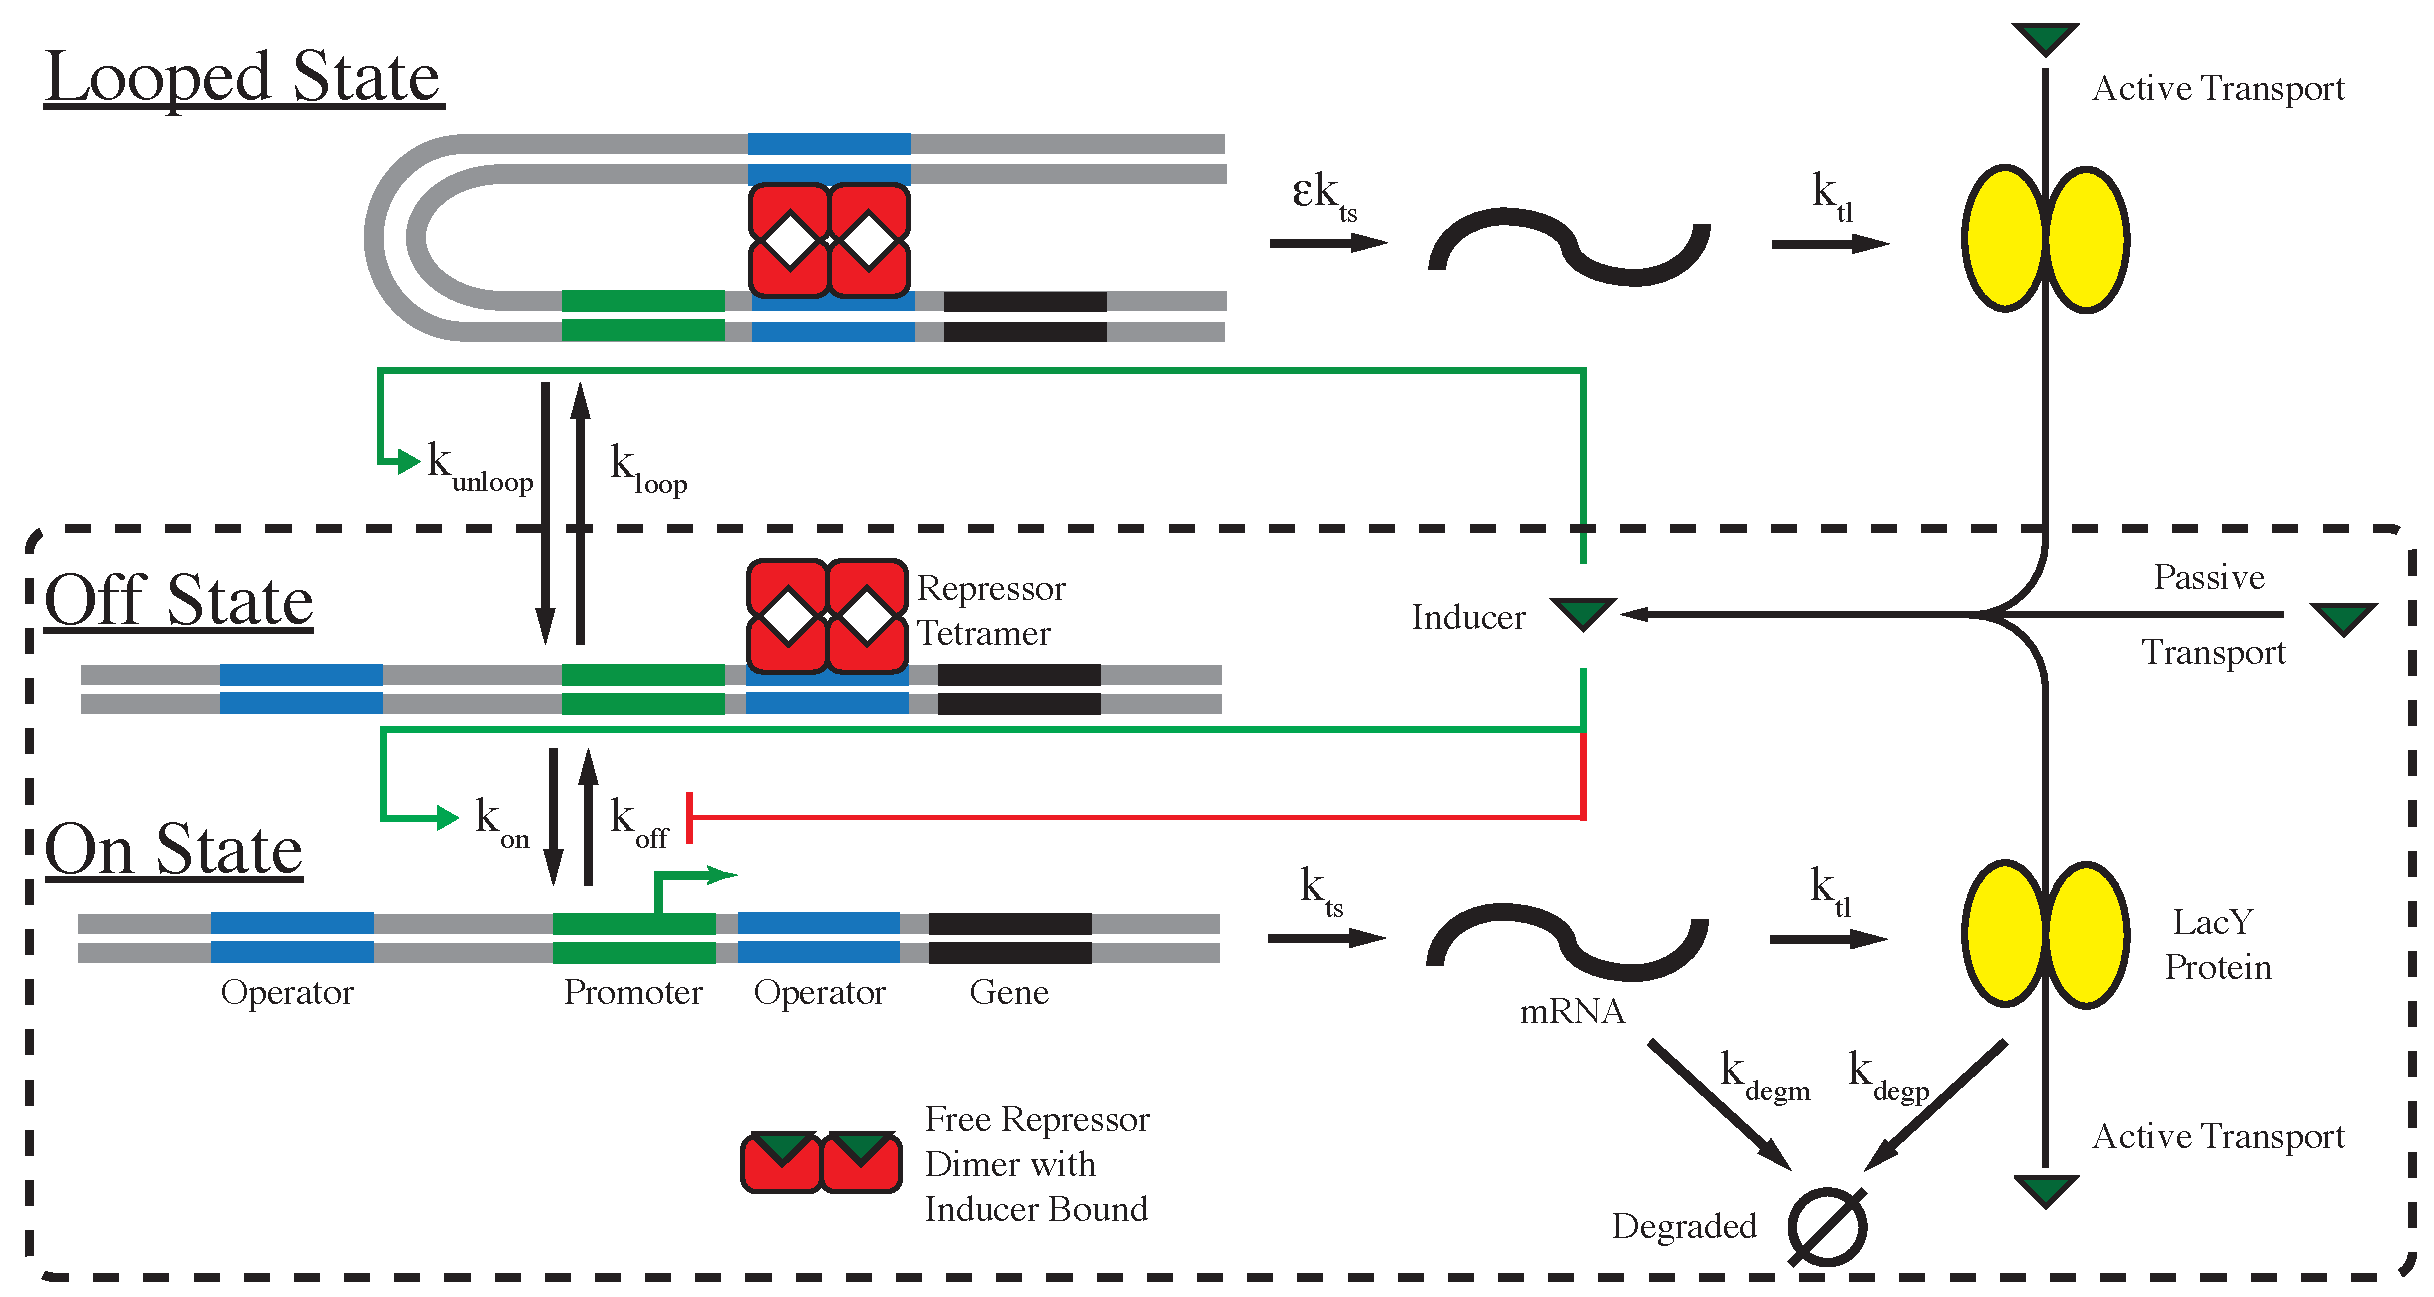
\includegraphics[width=0.8\textwidth]{Figures/LacThreeState.pdf}
        \caption{A schematic of the {\emph lac} switch with a simple two-state model \cite{Roberts2011nci} (shown in the dotted box) and the full three-state model published subsequently \cite{Earnest2013dli}. In the two-state model, the repressor sits on the operator region just downstream from the promoter and prevents the polymerase from binding.  However, when an active inducer (in this case an analog of lactose) is available, it binds to the repressor inducing it to unbind and enabling the gene to produce mRNA.  The mRNA encodes for a transport protein that actively transports more inducer into the cell, which allows the gene to be on for a longer period of time. Figure from \cite{Peterson2013}.} \label{fig:lacSwitch}
\end{figure}

\begin{figure}[h!]
  \centering
        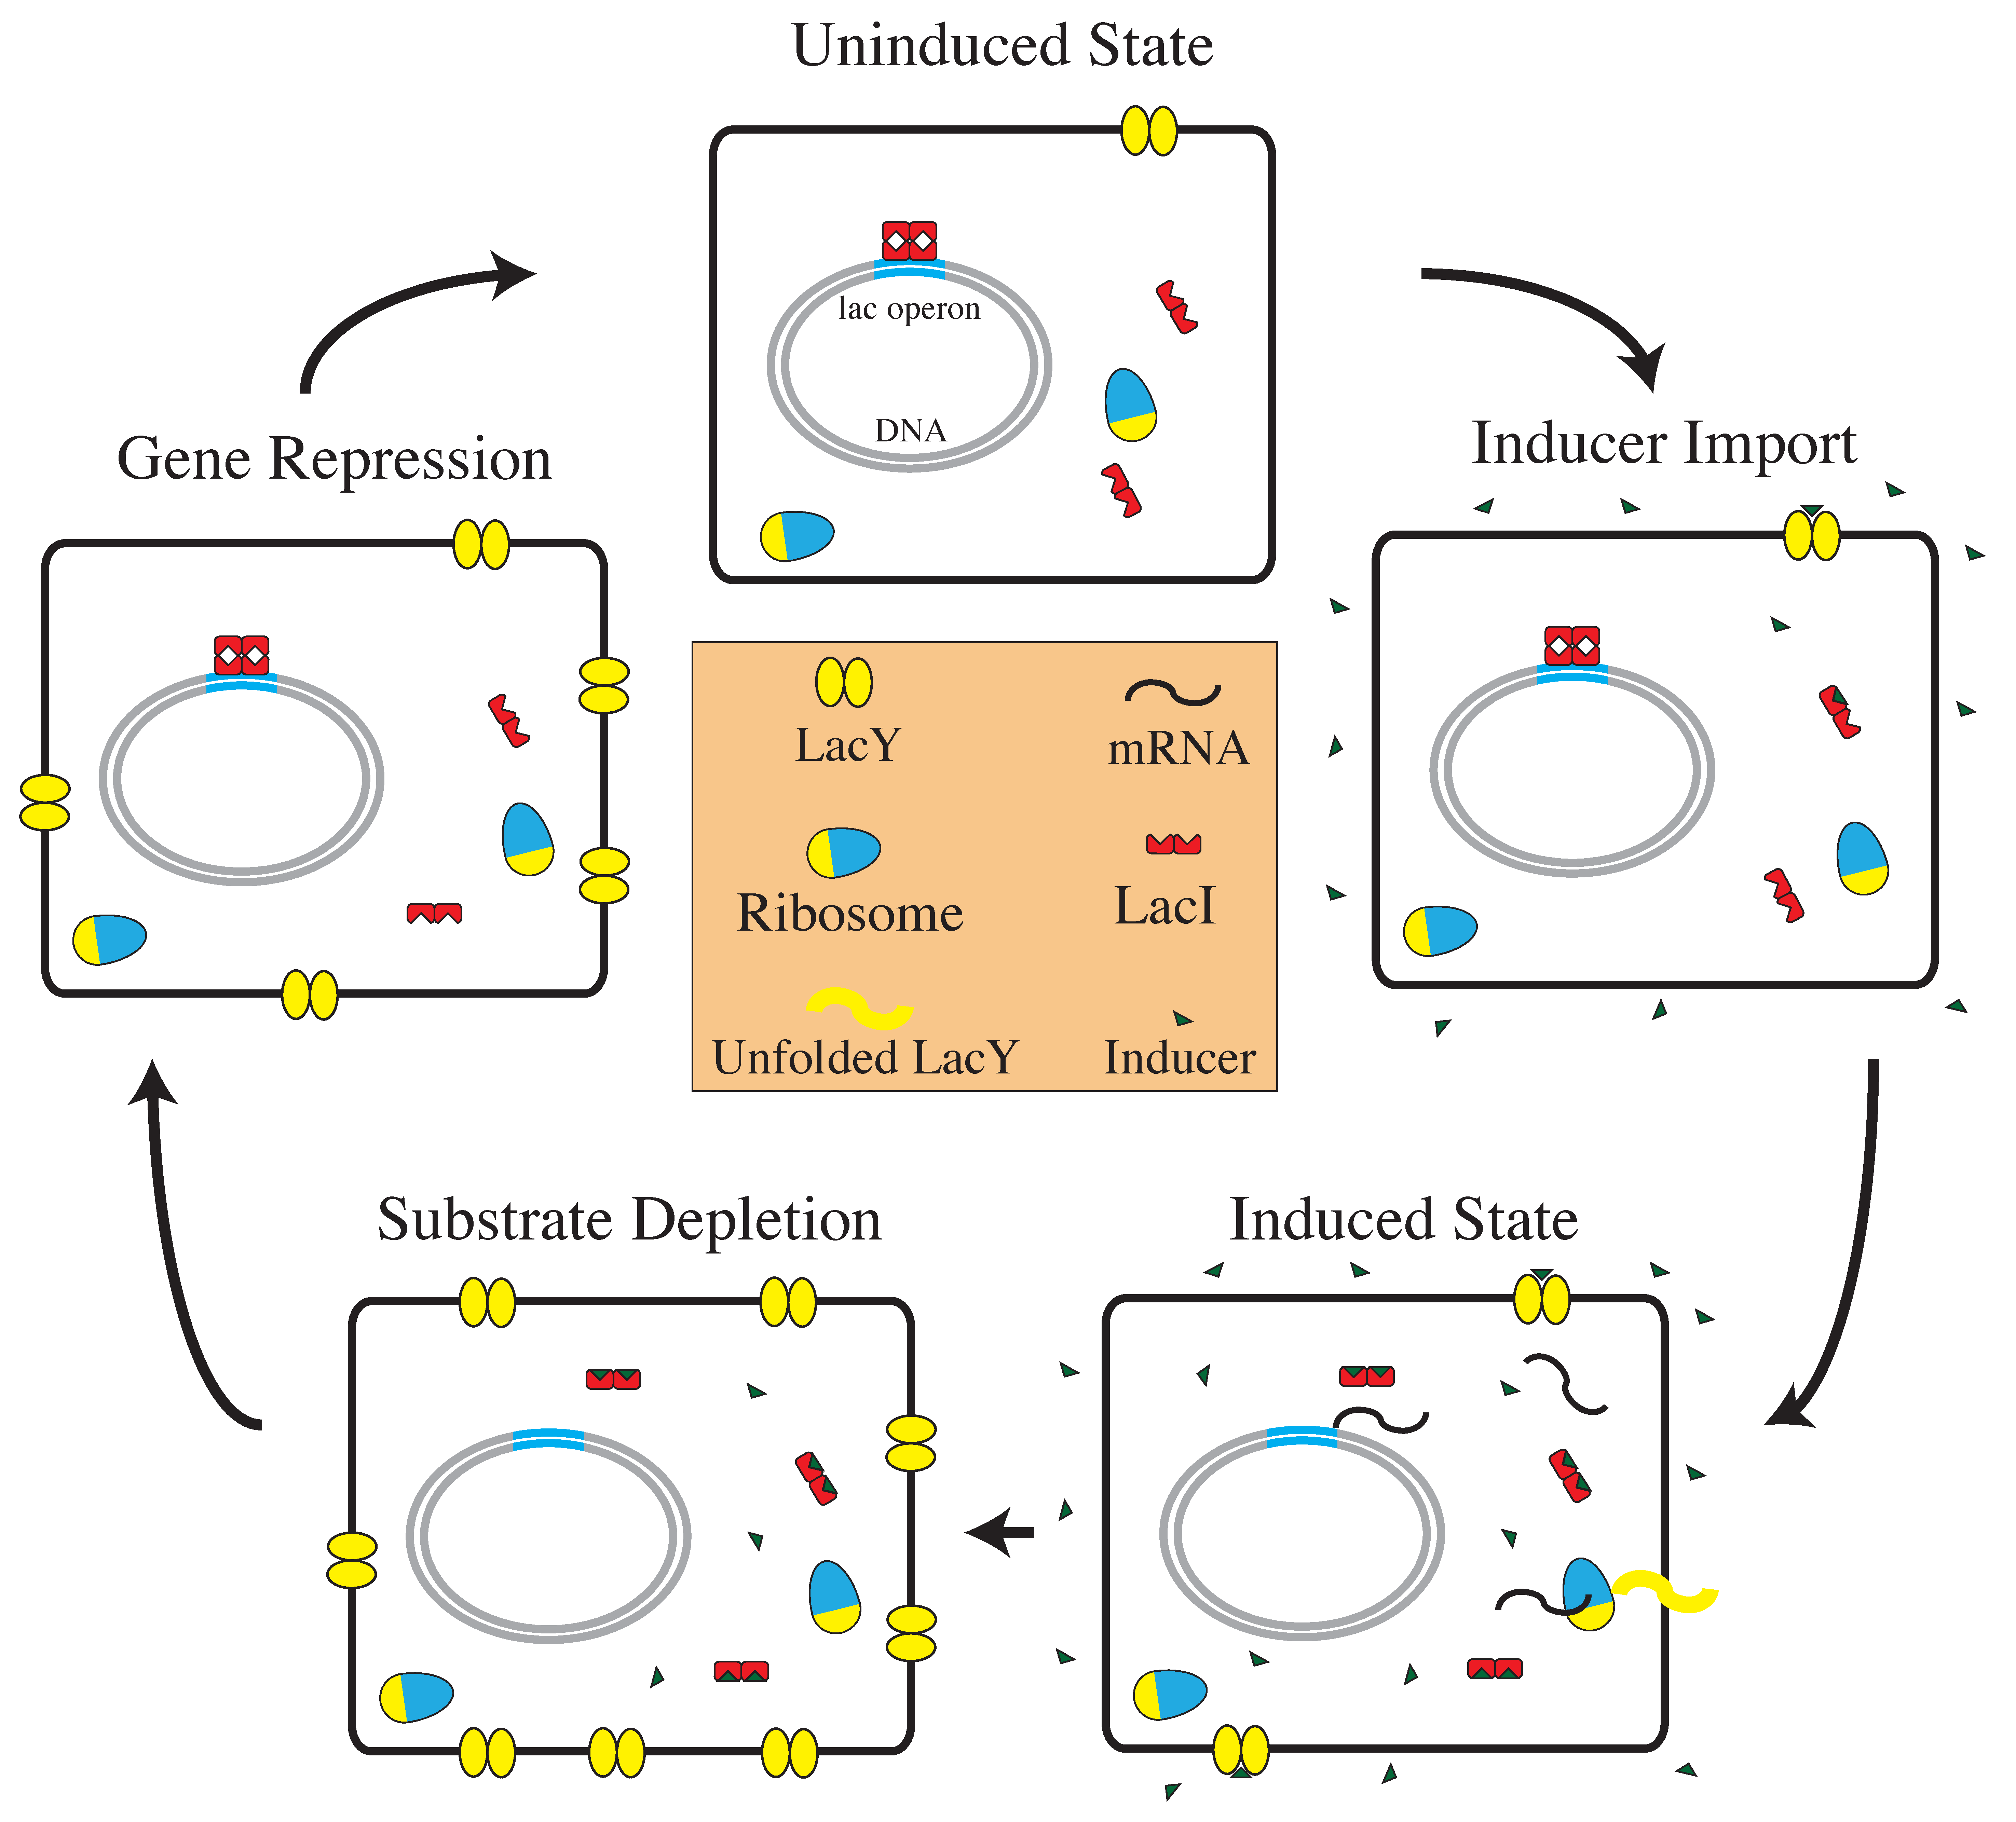
\includegraphics[width=0.7\textwidth]{Figures/LacSchematic.pdf}
        \caption{A cycle showing five different processes that occur during the induction of the switch. Figure from \cite{Peterson2013}.} \label{fig:lacLife}
\end{figure}

For simplicity, we will consider only the two-state {\it lac} model.  Even in the more limited two-state model, several salient features were discovered including deficiencies in previous models and the extent to which stochasticity played a role \cite{Roberts2011nci}.  We will initially examine the system under the well stirred assumption and then move on to a spatially resolved model.

\subsection{Well-Stirred}

The {\it lac} switch model has 23 reactions with 7 different substrates.  Setting up of the simulation is very similar to the previous example, so only the differences will be noted.  Specifically, this section is designed to show you how custom post-processing can be achieved.  The code to set up the simulation can be seen in Listing \ref{lst:lacCME}.

\lstinputlisting[style=customPy, caption={\texttt{tut2.1-lac2stateCME.py} --- Code to set up and execute the {\it lac} two-state model with CME.}, backgroundcolor=\color{mygray}, label=lst:lacCME]{CodeFiles/tut2.1-lac2stateCME.py}

This simulation will take a bit longer than the previous one. It is likely it will take between 5 and 30 minutes.  \\

This time we have used a pre-processing command to plot the network of reactions.  Namely, the command \texttt{plotCMEReactionNetwork(sim, filename="lacGraph.gml")} will create a graph file called `lacGraph.gml' which can be opened with a program like Gephi (\url{https://gephi.org})  or Cytoscape (\url{http://www.cytoscape.org}), resulting in an image like that seen in Figure \ref{fig:lacGraph}.  The use of these softwares is beyond the scope of this guide and we suggest you see the webpages for use. \\

The next difference is that we use a different solver, namely the Next Reaction solver, which is slightly less efficient than the Gillespie SSA solver used in the previous example \cite{Roberts2013lmh}.  Next, we have a loop that plots the traces of the messenger `mY' and the count of the protein `Y' as a function of time.  This line produces 100 files and can be commented out if uneccesary.  \\

Finally, we have a set of code that is custom post-processing that does a cluster on the data to get a heat map of the phase-space traversed by the messenger and protein over all the replicates. This demonstrates four other functions that are particularly important.  Generally, when your want custom post-processing you will be interacting with the file for a while, so use \texttt{openLMFile(filename)} to get a handle to the file.  Do not forget to call \texttt{closeLMFile(handle)}, or your data file could be corrupted.  Next, you will almost undoubtably want the time trace so call \texttt{getTimesteps(handle)} to get an array of the simulation timestep times.  Finally, you can get different species time traces using the function \texttt{getSpecieTrace(handle, specie, replicateNumber)}.  The rest is just standard Python, NumPy and matplotlib code.  A representative example can be seen in Figure \ref{fig:lacBursts}. \\

\begin{figure}[h!]
  \centering
        \includegraphics[width=0.5\textwidth]{Figures/LacGraph.pdf}
        \caption{A graph showing the possible interconversions of each species in the system.  The nodes are colored by initial count and the edges by the source node.  Self edges are shown as loops.} \label{fig:lacGraph}
\end{figure}

When examining a representative time trace one will notice a few interesting features (Figure \ref{fig:lacBursts}). Particularly, mRNA tend to be formed in bursts, which correspond to when a gene is `on' (no repressor is bound).  Correspondingly, there are large increases in the protein count during these times, until the mRNA degrades.  One can also map the phase space that is accessed by the simulations.  Averaging over 100 simulations over the first hour, and plotting protein (LacY) versus mRNA, one notes that there are two major populations (Figure \ref{fig:lacHeatmap}).  This heat map was generated with the custom post-processing code under the label ``Custom Post-Processing" in Listing \ref{lst:lacCME}.

\begin{figure}[h!]
  \centering
        \includegraphics[width=0.6\textwidth]{Figures/LacBursts.png}
        \caption{A single time trace from a single replicate showing the mRNA and Protein number over an hour period.  } \label{fig:lacBursts}
\end{figure}

\begin{figure}[h!]
  \centering
        \includegraphics[width=0.6\textwidth]{Figures/LacYmRNAHeatmap.png}
        \caption{The logarithm of the count of times the state (number of protein and number of messenger) was traversed over the time series averaged over 100 simulations for the first hour of simulation. Two clusters are clear in the map, one close to 0 mRNA and 50 protein and other with about 100 protein and 10 mRNA.} \label{fig:lacHeatmap}
\end{figure}



So now that you have a working understanding of how to use pyLM to do more complex tasks, try to answer a few of these questions:
\begin{enumerate}
\item What effect does the concentration of inducer have on the time to the cell turning `on'?
\item How long would it take for a cell to become very induced (about 2000 copies of the protein)?  Hint: try only a few simulations as they become slower after a very long time as species counts add up.
\item What would happen if the mRNA were longer lived, or if there were much larger bursts?
\item What effect would the extra looped state in the diagram above have on the switching time?
\item What would happen if protein did not degrade (dilute) on the timescale of a cell cycle?
\end{enumerate}


\subsection{Spatially Resolved} \label{sec:lacRDME}
With this introduction to the {\it lac} switch, we can now move on and see how spatial inhomogeneity can affect stochasticity in the system.  This section will take you through setting up your first spatially resolved simulation. Again, this was a simulation from \cite{Roberts2011nci}. The code to run this simulation can be seen in Listing \ref{lst:lacrdme}. \\

\lstinputlisting[style=customPy, caption={\texttt{tut2.2-lac2stateRDME.py} --- Code to set up and execute the {\it lac} two-state model with RDME.}, backgroundcolor=\color{mygray}, label=lst:lacrdme]{CodeFiles/tut2.2-lac2stateRDME.py}
 
The Python script will set up a cell with realistic crowding, internal and external inducer.  First off, spatial simulations require a lattice spacing to be defined.  This spacing is the side length for the volume that is assumed to be ``homogeneously" stirred (which allows CME to be applied in each subvolume). While this number can be too large, or two small and the CME assumption breaks down, the discussion of this is beyond the scope of this tutorial.  Eight, 16 and 32 nanometers are all fairly common lattice spacings.  Se then define the overall volume of the simulation.  In this case, we have created a cuboid shaped region with an aspect ratio of 2:1 (Lattice Microbes only supports cuboid shaped simulations).  \\

At this point, let us take a look at the anatomy of an RDME simulation.  A schematic of one is shown in Figure \ref{fig:rdmeschematic}.  As we have already described subvolumes and the overall simulation domain, there are only a few things to note. In Lattice Microbes, particles live in a subvolume, and the actual location within the subvolume is not known, but we can think of a particle as living in the center for simplicity.  What happens as time advances in the simulation is that particles within a subvolume can react, either by themselves or with other particles, or they can diffuse to one of the 27 (or fewer) direct neighboring subvolumes. At the current state, Lattice Microbes can support 8 different particles at a given site, with a total of 256 possible species/particle types.  Therefore the maximum occupancy of the total simulation domain is $8\times subvolumes$.  In practice, due to the algorithm, you will want to keep this number below 10\% of the total allowable occupancy. \\

Within the overall simulation domain there is a notion of regions. Regions are associated with a particular `site type'.  These could be things like a membrane or the cytoplasm, or something completely not biologically related. All the subvolumes assigned a site type that defines what can happen in that volume.  Regions are defined with possible chemical reactions that can occur in them, as well as what type of particles can diffuse into and out of them, as well as the diffusion rate into/out of and between these sites.  For instance, one protein might diffuse onto a membrane and have a lower diffusion rate on the membrane than in the cytosol.  Or a particular reaction may only occur in the cytosol.  Therefore, regions allow us to define what particles can do.  \\

However, regions need not be contiguous space.  As shown in the figure, there are two areas in the simulation that are the red region, and one that is the purple.  Therefore, all the reactions that can occur in one of the red region can also occur in the other even though they are not connected spatially.  This concludes our brief aside on the anatomy of an RDME simulation.\\

\begin{figure}[h!]
  \centering
        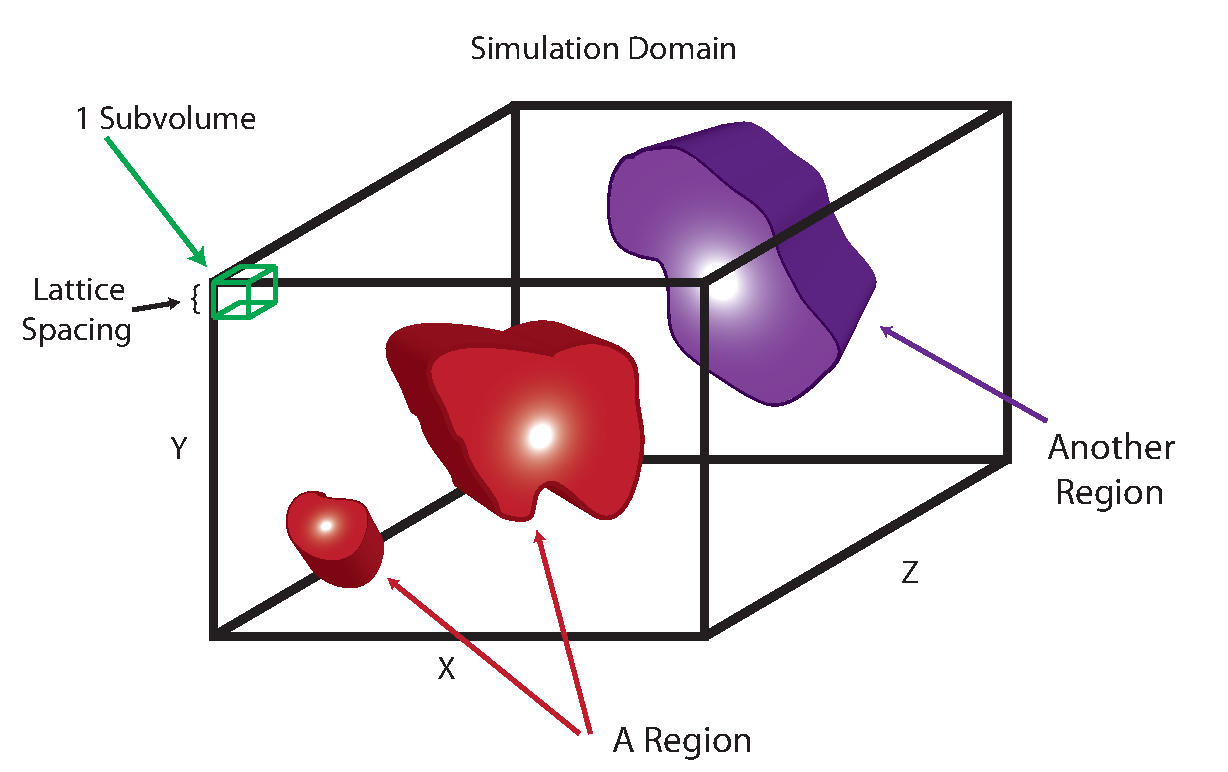
\includegraphics[width=0.7\textwidth]{Figures/RDMESchematic.pdf}
        \caption{A schematic of a hypothetical RDME simulation.} \label{fig:rdmeschematic}
\end{figure}

From an analysis of the previous code, it can be seen that one DNA particle `O' is placed (in this case randomly in the volume) along with a number of lac proteins `Y' that end up randomly on the membrane, nine repressor dimers `R2' and quite a few internal and external inducer molecules. Simulation parameters are specified and the simulation then runs for 10 minutes.  On a single GPU, this simulation takes about 32 hours to run, so you may want to get a coffee while it runs.  Alternatively, we have included a copy of the simulation results in the tutorial files and you can run the script with the \texttt{sim.run(filename...)} line commented out, and all the other code will work perfectly.  A similar figure to that plotted in the previous section is created with the same plotting command. \\

Perhaps more interesting, however, than this process is the visualization.  If you installed Lattice Microbes and the plugin for VMD, you will be able to open spatially resolved simulations.  To start, open up VMD, then load the file into the dialog box.  The result should look something like that seen in Figure \ref{fig:openDiag}; if ``Lattice Microbes" is not the file type, then the plugin is not installed correctly---please see the Lattice Microbes User Guide.  At first, the simulation will look rather boring, like that in Figure \ref{fig:firstOpen}.  The spherocylinder was drawn to show the shape of the cell, and several other shapes can be drawn, including cubes, spheres, etc.  Delete this by going to the ``Tk Console" in the ``Extensions" menu and entering the command \texttt{graphics top delete all} to reveal just the particles. \\

\begin{figure}[h!]
  \centering
        \includegraphics[width=0.5\textwidth]{Figures/openDialog.png}
        \caption{An example of the open dialog box in VMD.} \label{fig:openDiag}
\end{figure}

\begin{figure}[h!]
  \centering
        \includegraphics[width=0.7\textwidth]{Figures/InitiallyLoaded.png}
        \caption{A Lattice Microbes simulation initially loaded.} \label{fig:firstOpen}
\end{figure}

Next, we should pretty the simulation up some, as every particle is loaded the same color.  Open the ``Graphical Representations" tool from the ``Grpahics" menu and create representations similar to what you seen in Figure \ref{fig:graphicR}a.  In VMD each particle is known by a `type' which correspond to the order you registered species with the simulation via the \texttt{defineSpecies()} function in pyLM starting with 0 as the first index.  You will probably have to play with the ``Sphere Scale" to see all the particles. In this case, van Der Waals (``VDW") representation was used, but the ``Points" representation is equally useful.  \\ 

\begin{figure}[h!]
  \centering
          \begin{subfigure}[b]{0.29\textwidth}
          \includegraphics[width=\textwidth]{Figures/GraphicsRep.png}
        \end{subfigure}
        \begin{subfigure}[b]{0.68\textwidth}
          \includegraphics[width=\textwidth]{Figures/PrettiedView.png}
        \end{subfigure}
        \caption{a) Graphics Representation window showing what one such particle representation might look like. b) A view showing external inducer (red), internal inducer (gray), {\it lac} permease protein (blue), {\it lac} repressor (cyan) and the DNA particle (green).} \label{fig:graphicR}
\end{figure}

This should result in a view similar to what you seen in Figure \ref{fig:graphicR}b.  From here you can use the slider in the ``VMD Main" window to play through the frames of the movie.  Play around to see what else you can do.  \\

Now, often you will want to make sure the simulation is set up correctly by checking the site locations. VMD does not automatically load these, but it can be configured to load them.  Close VMD and reopen the program.  Before loading the simulation file, run from the console the following commands:

\begin{verbatim}
set env(LM_CREATE_OBSTACLE_ATOMS) 1
set env(LM_CREATE_SITE_ATOMS) 1
\end{verbatim}

Site types are named ``site" in VMD and can be selected similar to the way shown in Figure \ref{fig:repSites}.  The figure also demonstrates how to cut through the simulation using the selection ``x $<$ 51000".  In VMD the natural units are in angstroms, so the simulation is about 10240 angstroms  in x and y and 20480 in z.\\

\begin{figure}[h!]
  \centering
        \begin{subfigure}[b]{0.3\textwidth}
          \includegraphics[width=\textwidth]{Figures/RepSites.png}
        \end{subfigure}
        \begin{subfigure}[b]{0.69\textwidth}
          \includegraphics[width=\textwidth]{Figures/Sites.png}
        \end{subfigure}
        \caption{a) An example of a graphic representation of the site types. b)  Here the extracellular (also called default) is shown in gray, the membrane, which is about 2 sites thick, is shown in blue and the cytoplasm is shown in red.  Both the extracellular and the membrane are cut only show those with x less than 5100 angstroms.} \label{fig:repSites}
\end{figure}

One particular note of interest is that VMD automatically loads the first replicate, if more than one replicates were run.  In order to load a different replicate, you must follow the procedure for showing obstacle and site types just mentioned but with the Tk Console command:

\begin{verbatim}
set env(LM_REPLICATE) #
\end{verbatim}

Where the \# symbol is the replicate number.  Lattice Microbes files are standard HDF5 files, meaning they can be opened with HDFView (which is available from \url{http://www.hdfgroup.org/HDF5/}) and other features of the simulation can be inspected such as data layout, parameters, etc.  However, this is an advanced topic and beyond the scope of these tutorials. The user is, however, encouraged to explore the file if they are curious.  \textbf{Note: Do not open a Lattice Microbes file while the simulation is running!  In rare cases this can cause the data to be corrupted. If you must, we recommend you make a copy of the simulation file and open the copy.} \\

This concludes our brief introduction to spatially resolved simulations in Lattice Microbes.  Much additional functionality for setting up RDME simulations exists and can be found in the Lattice Microbes Reference Guide for pyLM available at the website.

%%%%%%%%%%%%%%%
% Section: Command Line %
%%%%%%%%%%%%%%%
\section{Debugging and Command Line Execution}
At this point, it is appropriate to address two topics that will no doubt be required if you use Lattice Microbes to solve anything but a toy problem.  This section describes the process for debugging simulations as well as how to invoke Lattice Microbes simulations from the command line, which is useful when running on supercomputers.  

\subsection{Debugging}

Sometimes a simulation will not work on the first try.  Python sometimes has the downfall of being too kind to errors, and we as programmers are sloppy.  As such, it may fail without a word and not perform the actions you requested.  Therefore, you will want to be able to debug what is going on in pyLM as it performs its task.  It provides this capability through a Python ``logger" which can be activated in the script.  We recommend you always activate this functionality when you are designing a simulation and then deactivate it when running production runs.  To enable the logging, merely add the following code to your simulation: \\

\begin{lstlisting}[style=customPy, caption={Code to enable debugging output in pyLM.}, backgroundcolor=\color{mygray}, label=lst:debug1]
from pyLM import LMLogger
LMLogger.setLMLogConsole(logging.WARNING)
\end{lstlisting}

Five levels of debugging information are available; listed in order of increased output: \texttt{logging.DEBUG}, \texttt{logging.INFO}, \texttt{logging.WARNING}, \texttt{logging.ERROR}, \texttt{logging.CRITICAL}.  Different levels are used throughout pyLM and pySTDLM to inform the user what is going on, as well as any other errors or warning that might have occurred.  As an example we have included a test file with an error in Listing \ref{lst:debug3}.  Try running the code with the various different levels to try to identify the error.

\lstinputlisting[style=customPy, caption={\texttt{tut2.3-debugging.py} --- Code with an error.}, backgroundcolor=\color{mygray}, label=lst:debug3]{CodeFiles/tut2.3-debugging.py}

In addition, you may want to add your own debugging to the output.  As such you can simply add lines such as:

\begin{lstlisting}[style=customPy, caption={Custom debugging output.}, backgroundcolor=\color{mygray}, label=lst:debug2]
LMLogger.error("This is an error: %d"%var)
LMLogger.info("General info for me...")
LMLogger.warning("Are you sure you want to do this: %s"%"Something dangerous")
\end{lstlisting}


\subsection{Command Line}

While launching the simulations from within a Python script is what you will want to do during testing, it may not be the best way to launch the code for a production run.  For example, some clusters and supercomputers do not have the correct Python environment, or allow interpreted languages to be run as the primary executable.  Therefore, you may want to launch your job from the command line using the \texttt{lm} executable.  Luckily, you can prototype your simulation in Python as discussed before, then comment out the \texttt{sim.save(...)} and \texttt{sim.run(...)} commands, run the simulations on a supercomputer, then run the Python script on the already produced output, to leverage the power of scripting for custom post-processing.  \\

Running Lattice Microbes from the command line can be fairly straightforward.  For example, running the simulation in Listing \ref{lst:lacrdme} one would execute the following command:

\begin{verbatim}
lm  -r 0-2 -sp -sl lm::rdme::MpdRdmeSolver -f T2.2-lac2state.lm
\end{verbatim}

To dissect the command, the \texttt{-r 0-2} indicates to run three replicates with indices 0, 1 and 2, \texttt{-sp} indicates the simulation is spatially resolved (i.e. RDME), \texttt{-sl lm::rime::MpdRdmeSolver} is the particular solver to use to sample the stochastic equations and \texttt{-f T2.2-lac2state.lm} indicates the file that should be used.  \\

On a supercomputer or cluster where multiple CPU's and/or multiple GPU's are to be used, you may need to specify additional arguments.  For example, on a system with 2 GPU's per node, and 8 CPU cores, you could split up 16 replicates as such:\\

\begin{verbatim}
mpirun -np 8 lm -r 0-15 -sp -sl lm::rdme::MpdRdmeSolver -gr 1/16 \
       -cr 1/2 -f T2.2-lac2state.lm
\end{verbatim}

which will dedicate one sixteenth of a GPU and a half of a CPU core to each replicate.  Alternatively, the simulations will be run in two sets if you only run: 

\begin{verbatim}
mpirun -np 8 lm -r 0-15 -sp -sl lm::rdme::MpdRdmeSolver -gr 1/8 \
       -cr 1 -f T2.2-lac2state.lm
\end{verbatim}

However, it should be noted that usually on large supercomputers or for complex jobs you may want a dedicated CPU for the data input/output thread.  This thread is launched by default per simulation, so you could subtract that number from your total CPU cores.  

To get a complete listing of the commands run \texttt{lm -h} which should give a prompt similar to:

{\scriptsize
\begin{verbatim}
Usage: lm (-h|--help)
Usage: lm (-v|--version)
Usage: lm [OPTIONS] (-l|--list-devices)
Usage: lm [OPTIONS]
Usage: lm [OPTIONS] (-s|--script) script_filename [(-sa|--script-args) script_arguments+]
Usage: lm [OPTIONS] [SIM_OPTIONS] (-f|--file) simulation_filename 

OPTIONS
  -c num_cpus       --cpu=num_cpus               
  		The number of CPUs on which to execute (default all).
  -cr num           --cpus-per-replicate=num     
  		The number of CPUs (possibly fractional) to assign per replicate, e.g. "2", "1/4" (default 1).
  -g cuda_devices   --gpu=cuda_devices           
  		A list of cuda devices on which to execute, e.g. "0-3", "0,2" (default 0).
  -gr num           --gpus-per-replicate=num     
  		The number of cuda devices (possibly fractional) to assign per replicate, e.g. "2", "1/4" (default 1).
  -nc               --no-capabilities            
  		Don't print the capabilities of the CUDA devices.
  -nr               --no-reserve-core            
  		Don't reserve a CPU core for the output thread.

SIM_OPTIONS
  -r replicates     --replicates=replicates      
  		A list of replicates to run, e.g. "0-9", "0,11,21" (default 0).
  -sp               --spatially-resolved         
  		The simulations should use the spatially resolved reaction model (default).
  -ws               --well-stirred               
  		The simulations should use the well-stirred reaction model.
  -sl solver        --solver=solver              
  		The specific solver class to use for the simulations.
  -ck               --checkpoint=interval        
  		Enable checkpointing with the given interval as hh:mm:ss (default 00:00:00 -- disabled).
\end{verbatim}
}

%\subsection{SBML Files}
%To be completed...


%%%%%%%%%%%%%%%
% Section: The Min system %
%%%%%%%%%%%%%%%
\section{Advanced Post-Processing: The Min System}

In this section, we will use another popular stochastic simulation to demonstrate more advanced post-processing using Python.  In particular, we will use the Min protein system \cite{Loose2011pso,Fange2006nim}, shown schematically in Figure \ref{fig:minsystem}, that places the division plane in the center of the cell during division of {\it E. coli}.  As the system evolves from the initial state, an oscillation of the two proteins from one pole of the cell to the other at a frequency close to 1 per minute, with the MinE protein stimulating the detachment of the membrane bound MinD protein activating its ATPase activity.  One particular interesting fact is that certain mutants of {\it E. coli} show anomalous Min system behavior that cannot be captured with deterministic PDE simulations and require the use of stochastic simulation techniques like the RDME.

\begin{figure}[h!]
  \centering
        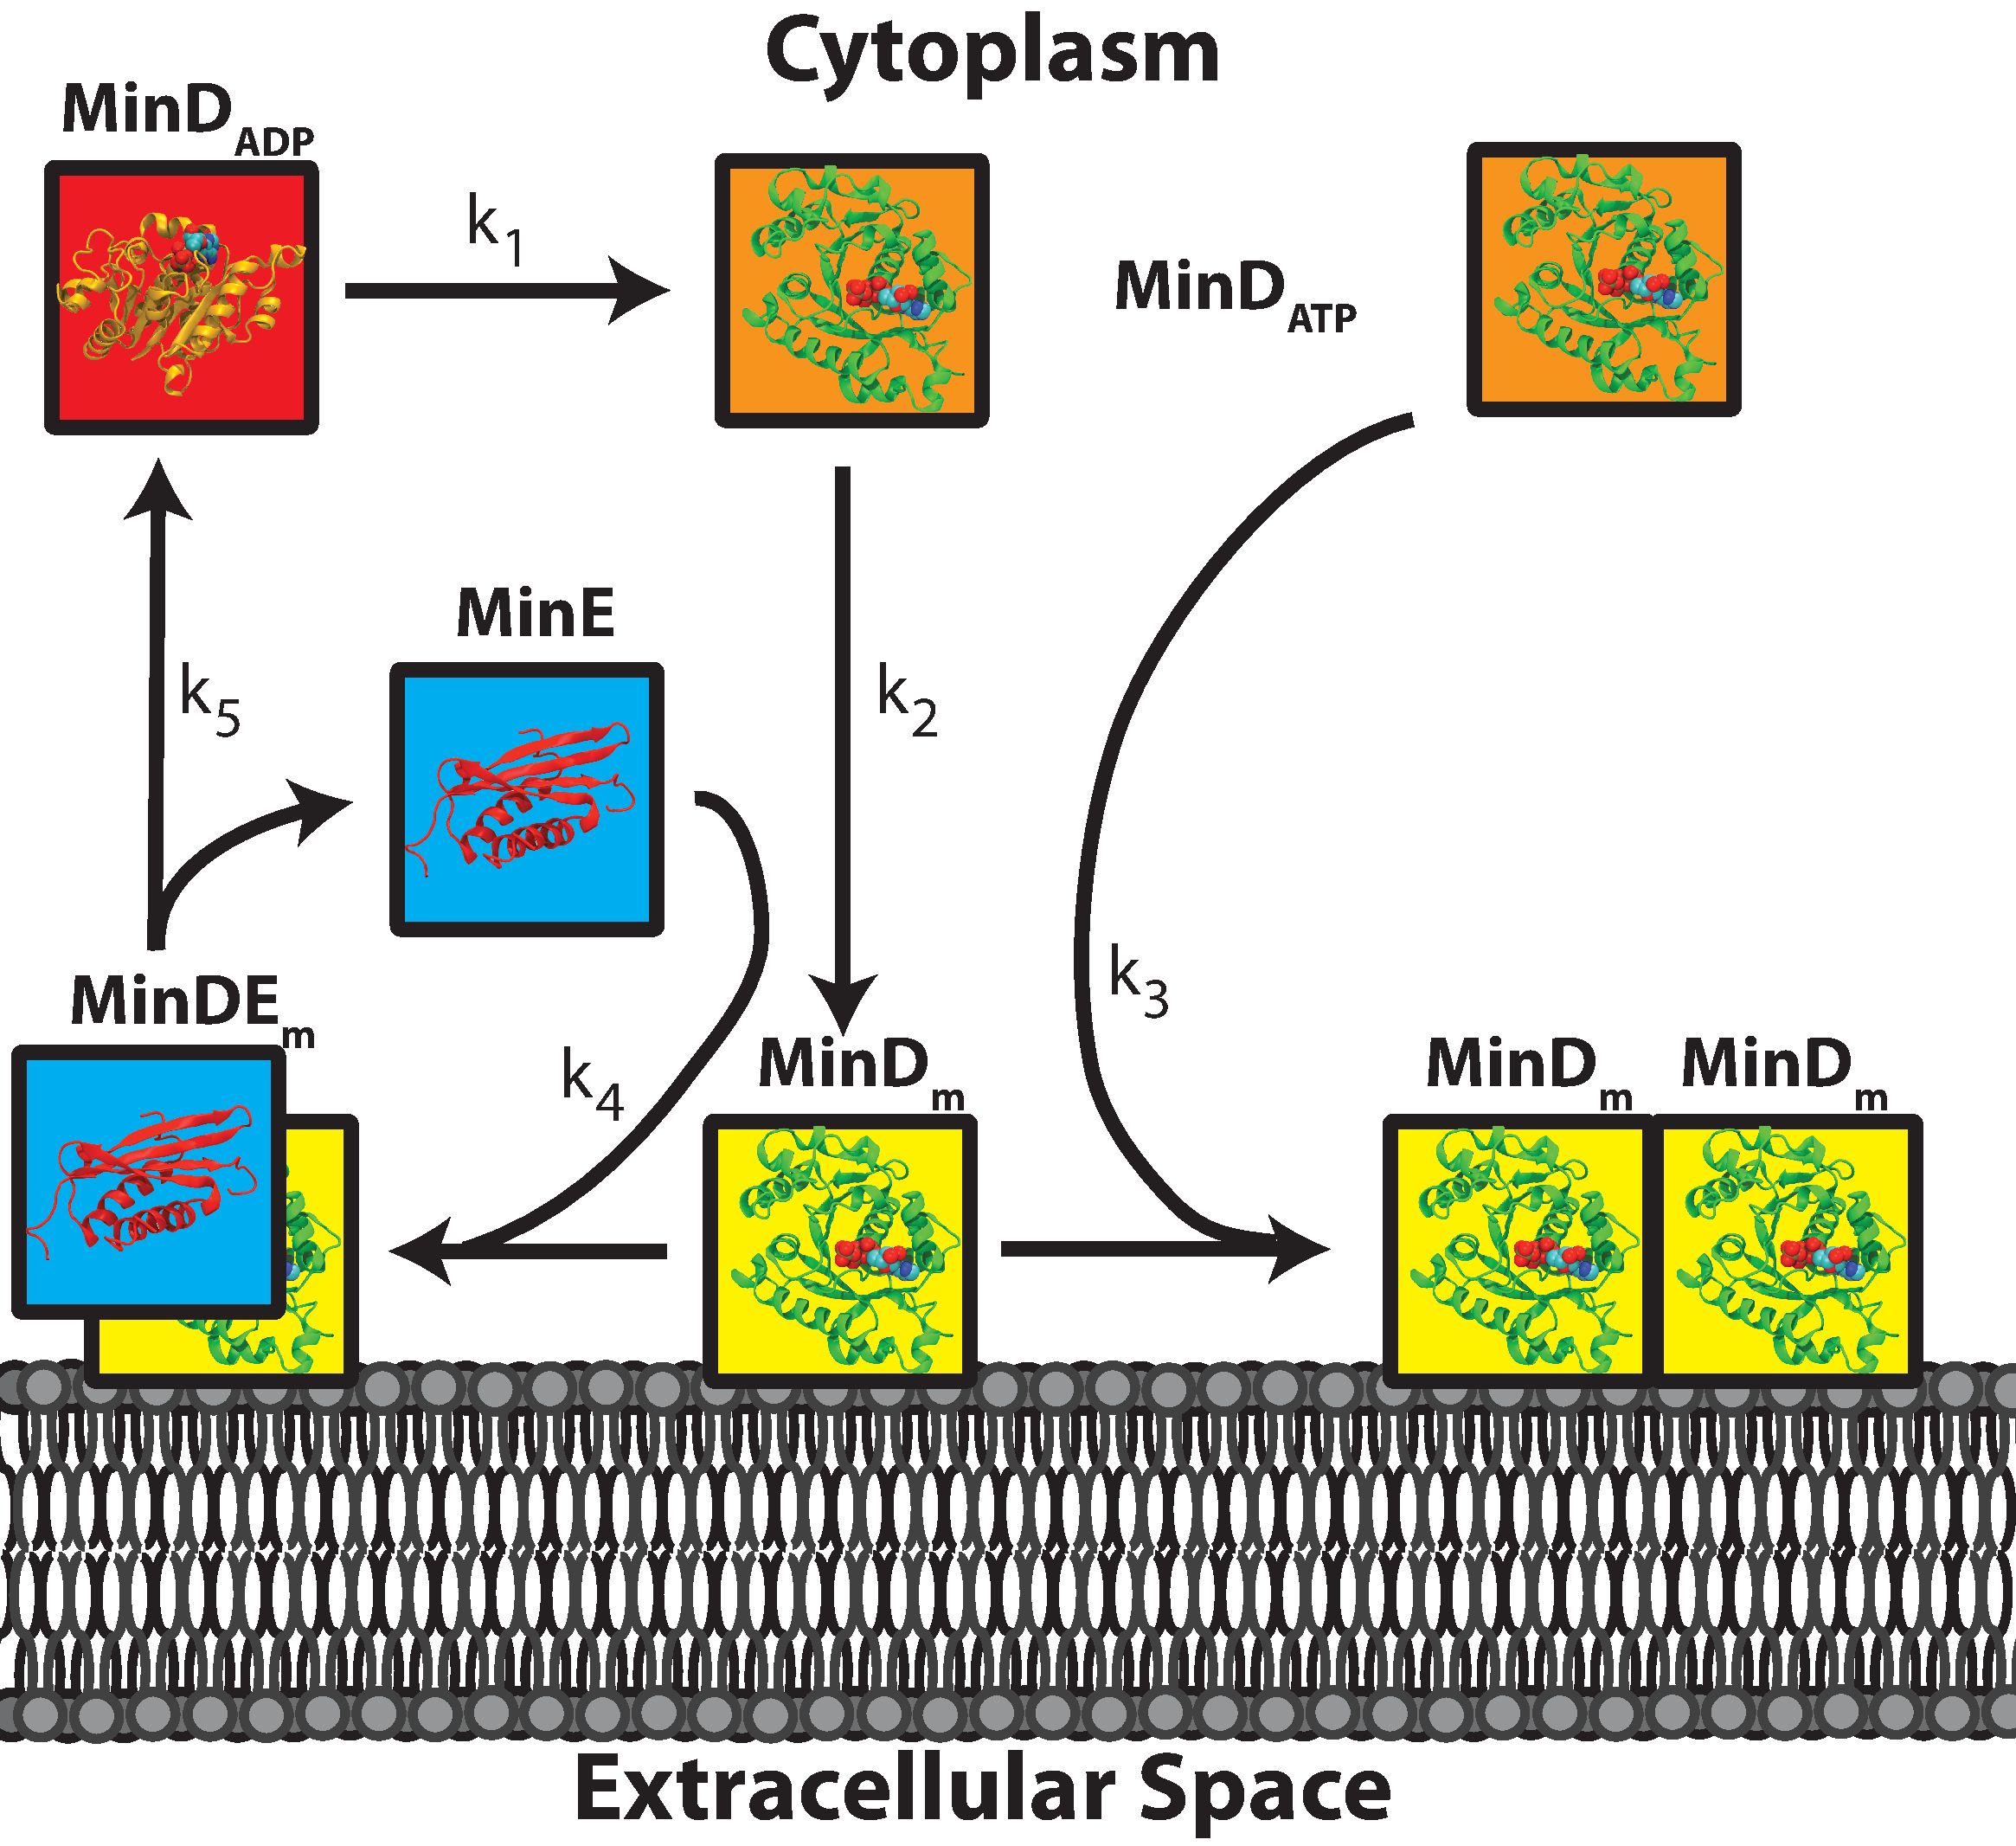
\includegraphics[width=0.5\textwidth]{Figures/MinDESystem.pdf}
        \caption{A schematic of the Min protein system model \cite{Peterson2013}.  ATP bound MinD attaches to the membrane and can long fields of bound MinD.  MinE binds to membrane bound MinE stimulating its ATPase activity and causing the MinD to leave the membrane where, once back in the cytoplasm, another ATP can replace the bound ADP.} \label{fig:minsystem}
\end{figure}

Again, the simulation setup is fairly easy, and this Min system is available as a standard reaction system in pySTDLM.  The code to setup up, run and analyze the simulation is shown in Listing \ref{lst:minsystemrdme}.  Everything before post-processing is similar to that in Section \ref{sec:lacRDME} so will not be discussed. 
%The first new command is used to plot the dynamics of a reaction network; it extracts the time course of each species and plots the values on the nodes of a dynamic graph. This graph, which has the extension `.gexf' is viewable in the Gephi program (\url{https://gephi.org}), and are similar to that seen in Figure \ref{fig:lacGraph}.  Three snapshots of the simulation are shown in Figure \ref{fig:mindegraph} showing the oscillation of population of MinD and MinE at different times.

\lstinputlisting[style=customPy, caption={\texttt{tut3.1-minsystem.py} --- Code to set up and execute the Min protein system with RDME.}, backgroundcolor=\color{mygray}, label=lst:minsystemrdme]{CodeFiles/tut3.1-minsystem.py}

\begin{figure}[h!]
  \centering
        \includegraphics[width=0.8\textwidth]{Figures/MinDESnapshots.png}
        \caption{Three times during the simulation showing membrane bound MinD (cyan) oscillating from pole to pole with MinE (red) trailing behind the wavefront.} \label{fig:mindegraph}
\end{figure}

The next two commands plot a kymograph of the occupancy of that (x,y) coordinate of the z slice as a function of time.  Currently, only slices in z are supported, but this will be expanded in a future release of pyLM.  The occupancy is computed as the number of sites that contain a particular particle divided by the total number of sites in that slice.   The kymograph for membrane bound MinD  can be seen in Figure \ref{fig:kymographs}.  

\begin{figure}[h!]
  \centering
        \includegraphics[width=0.5\textwidth]{Figures/mindm.pdf}
        \caption{End to end oscillations of the membrane bound MinD as the system progresses in time.} \label{fig:kymographs}
\end{figure}

%%%%%%%%%%%%%
% Section: Advanced Uses %
%%%%%%%%%%%%%
\section{Advanced Uses: Merging RDME with CME}

This section will show you how to use a feature of pyLM that allows custom control of the simulation states the simulation progresses.  In order to run the examples in this section your HDF5 library needs to have been compiled with the \texttt{--enable-threadsafe} option.  If the example exhibits random crashing, you will likely have to recompile your HDF5 library.  In this section we will create a subclass of the MPD RDME Solver class that will perform custom operations during at a specified time interval (in this case, every time the simulation state is written to file).  \\

\begin{figure}[h!]
  \centering
        \includegraphics[width=0.9\textwidth]{Figures/CombinedSchematic.png}
        \caption{A schematic of the combined RDME/CME simulation.  } \label{fig:advancedSchematic}
\end{figure}

This simulation mocks the production of a protein from its gene and the resulting consumption of a substrate by that enzyme (see Figure \ref{fig:advancedSchematic}).  To reduce the computational cost of carrying around many substrate and product molecules in the RDME lattice, they are treated as well stirred (i.e. the molecules are much smaller than the enzymes).  However, the translational machinery interactions are spatially resolved.  Finally, the products from the enzyme reaction are inserted into the RDME simulation domain as they are created, so that they could potentially interact with the DNA to create some sort of feedback (however, this case is not explicitly treated in this tutorial).  \\

The point of the tutorial is to highlight the extendability of the RDME solver in pyLM.  Right after turning on the logging, a new class is defined called ``MyOwnSolver" that extends the MPD RDME Solver.  A few of the internal variables are then created including initial timestep, species and time trace arrays.  The meat of the solver is in the function \texttt{hookSimulation(...)} which is a time-based interrupt to the Lattice Microbes simulation.  Essentially, this function is called every time a lattice is written (the same frequency as that set in \texttt{setLatticeWriteInterval(...)}).  The RDME simulation pauses, passes the current \texttt{time} and \texttt{lattice} to this function and pretty much any Python code can be executed.\\

\lstinputlisting[style=customPy, caption={\texttt{tut3.2-rdmecme.py} --- Code that shows how an RDME and CME simulation can be coupled using a time-based interrupt.}, backgroundcolor=\color{mygray}, label=lst:minsystemrdme]{CodeFiles/tut3.2-rdmecme.py}

So after simulating for a quarter of a second, the function is called and a new CME simulation for the enzyme catalysis is created.  As an input, it uses the current number of enzyme particles in the CME (which it determines by the function call \texttt{findParticle(low,high)}, where the low and high are indices into the defined species list).  The CME simulation rates and reactions are set and it is run using a system call \texttt{os.system(...)} using another instance of Lattice Microbes.  Currently, the \texttt{runSolver(...)} command cannot be used here as it conflicts with some threads, however this will be rectified in a later version.  Finally, when the CME simulation is completed, it reads the number of new product particles, adds them to the RDME simulation in random places using the \texttt{addParticle} call.  Finally, it copies the CME simulation particle traces to internal variables of the ``MyOwnSolver" class for use later.  \\

The rest of the code is fairly boiler plate setting up an RDME simulation and running it.  In this case we assume RNA is transcribed at about 70 nucleotides per second and protein is produced at about 40 amino acids per second.  We assume a protein of about 160 amino acids length, and pick some numbers for different rates.  Finally around line 170 some post processing occurs to plot out several traces using a system call to use Gnuplot.  \\

The results of the simulation can be seen in Figures \ref{fig:rdmecmecoupled} and \ref{fig:rdmecmetimetrace}.  While the results are relatively uninteresting, the code demonstrates how one would merge different types of kinetic methods.  For example, the CME could be replaced by a standard set of continuous ordinary-differential equations, or by a steady state method like flux-balance analysis (as was done recently \cite[Chapter~13]{BookChapter}).  Alternatively, one could implement a feedback system where the product particles caused the gene to be turned off with a certain probability. We encourage you to think outside the box and push our software to its limits. \\


\begin{figure}[h!]
  \centering
        \includegraphics[width=0.7\textwidth]{Figures/Coupled.png}
        \caption{A schematic of the combined RDME/CME simulation performed in this section where transcription/translation are spatially resolved and enzyme catalysis is assumed to be a well-stirred process.} \label{fig:rdmecmecoupled}
\end{figure}

This concludes our basic tutorials.  While we only covered a fraction of the possible functionality available in Lattice Microbes/pyLM, we think this is enough to enable you to begin using it.  Full documentation is available on the Lattice Microbes website. \\

\begin{figure}[h!]
  \centering
        \includegraphics[width=1.0\textwidth]{Figures/RDMECMETimetrace.png}
        \caption{Three times during the simulation showing DNA (green), RNA (red), protein (brown) and product molecules added to the simulation (pink).} \label{fig:rdmecmetimetrace}
\end{figure}

If you are interested in giving feedback or suggestions, please email the developers.  In addition, we look forward to contributions from the community.  Furthermore, if you publish any results based on simulations from Lattice Microbes, we ask that you notify us by sending a citation to your paper so that we can follow what work is being done with the code.  
